\begin{figure}[H]
    \centering
    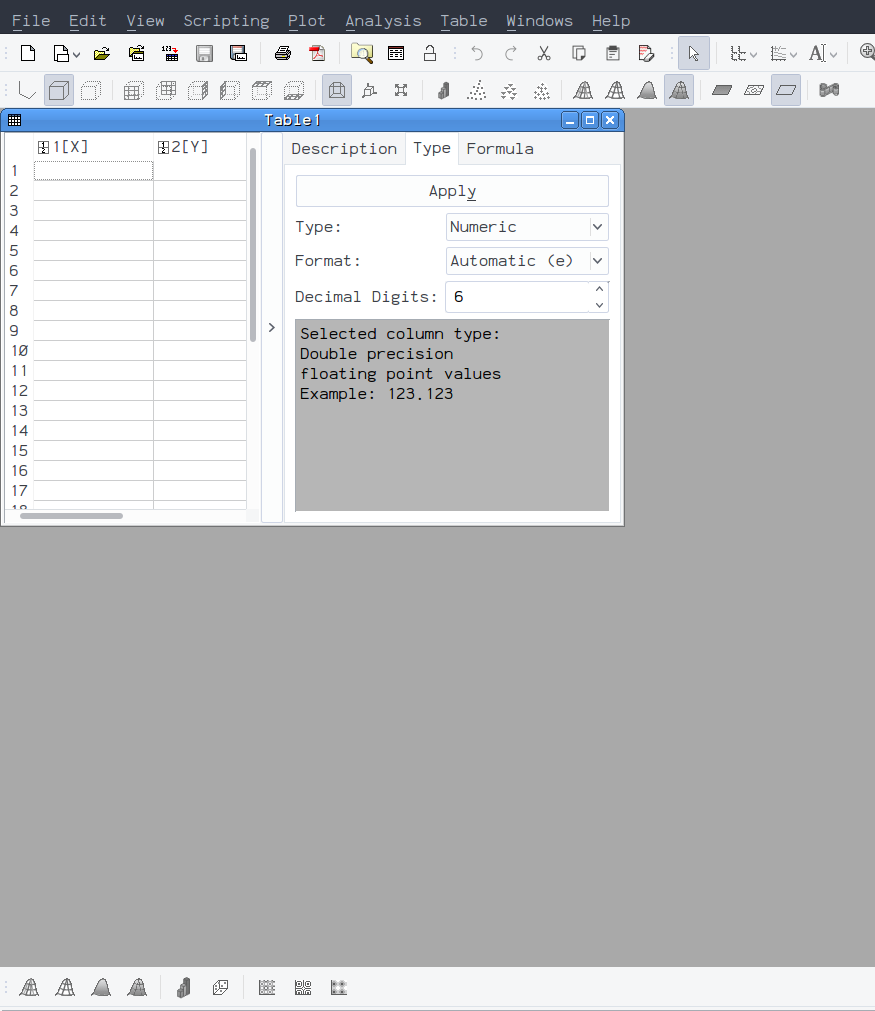
\includegraphics[width=0.6\textwidth]{basico/1mostra.png}

    \caption{Tela inicial do \software}
    \label{fig:basico:mostragem}
\end{figure}


% \subsection{Alterando a Fonte Padrão}

%     Como a fonte padrão do \texttt{Origin} não funciona muito bem com acentos e outros símbolos da língua portuguesa, é recomendado utilizar outra fonte nos gráficos. Nos exemplos a seguir será aplicada a fonte \texttt{Times New Roman}, que funciona com os acentos gráficos e é facilmente encontrada em qualquer máquina com \texttt{Windows}. Todo o processo é bem simples e está especificado na figura \ref{fig:basico:mudar_fontes}.

%     \begin{figure}[htbp]
%         \centering
%         \begin{subfigure}{0.45\textwidth}
%             \centering
%             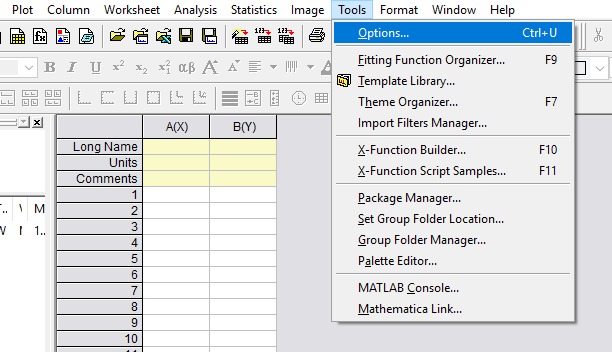
\includegraphics[width=\textwidth]{basico/2options.png}

%             \caption{Acesso às opções}
%             \label{fig:basico:options}
%         \end{subfigure}
%         ~
%         \begin{subfigure}{0.45\textwidth}
%             \centering
%             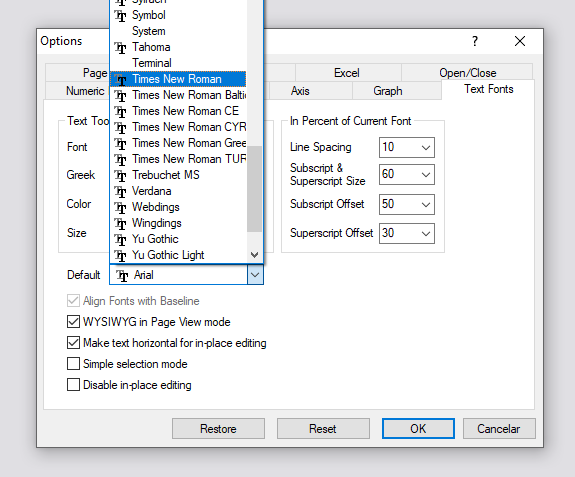
\includegraphics[width=\textwidth]{basico/3fonts.png}

%             \caption{Opção de fontes}
%             \label{fig:basico:fontes}
%         \end{subfigure}
%         \caption{Mudando a fonte padrão}
%         \label{fig:basico:mudar_fontes}
%     \end{figure}


\subsection{Importando os Dados} \label{sec:basico:import}

    Assim como no \texttt{Origin}, o \software tem um gerenciador de tabelas prórpio, apesar de simplificado, onde os dados podem ser apenas copiados e colados de outra tabela do \texttt{Excel}, \texttt{Google Planilhas}, \texttt{LibreOffice Calc} ou outra ferramenta do tipo. Quando os dados são importados assim, a formatação das linhas e colunas se matém. Outra opção é importar de arquivos de texto de campos separados, como o \texttt{CSV} e suas variações.

    \begin{lembrete}
        Cuidado com o separador decimal. Em português e outras línguas europeias é mais comum encontrar a vírgula [\texttt{,}] como separador da parte decimal do número, enquanto nos países anglofônicos é o ponto final [\texttt{.}] que define a parte fracionária e a vírgula serve para separar os milhares. Dependendo da configuração do \software e da formatação original dos dados, isso pode causar problemas de importação e os dados serão tratados como tipo \texttt{Text}.
    \end{lembrete}


\subsection{Configurando as Colunas} \label{sec:basico:renome}

    Por padrão, as colunas são criadas com letras com números. Para mudar isso, basta alterar as propriedades da coluna, que fica na parte direita da janela da tabela, como na figura \ref{fig:basico:colnome}. Além disso, se você importar os dados de um arquivo \texttt{.csv}, é possível utilizar a primeira linha como nome da coluna, o \textit{header}.

    Outra coisa importante é o tipo de dado da coluna. Para a construção dos gráficos, o desejado normalmente são dados de tipos numéricos ou, às vezes, datas. Porém, é possível que os dados estejam sendo tratados como texto, como no problema descrito na seção \nameref{sec:basico:import}. Por isso, deve se ter o cuidado de escolher o tipo certo, seguindo a figura \ref{fig:basico:coltipo}, antes e depois de importar os valores.

    \begin{figure}[htbp]
        \begin{subfigure}{0.45\textwidth}
            \centering
            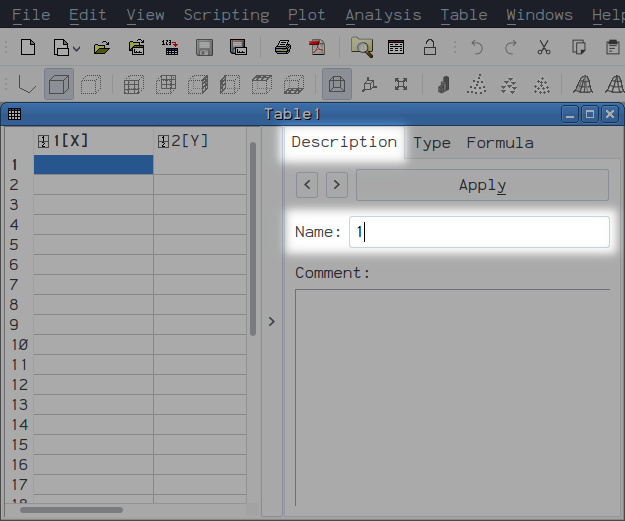
\includegraphics[width=\textwidth]{basico/3colnome.png}

            \caption{Nome da coluna}
            \label{fig:basico:colnome}
        \end{subfigure}
        ~
        \centering
        \begin{subfigure}{0.45\textwidth}
            \centering
            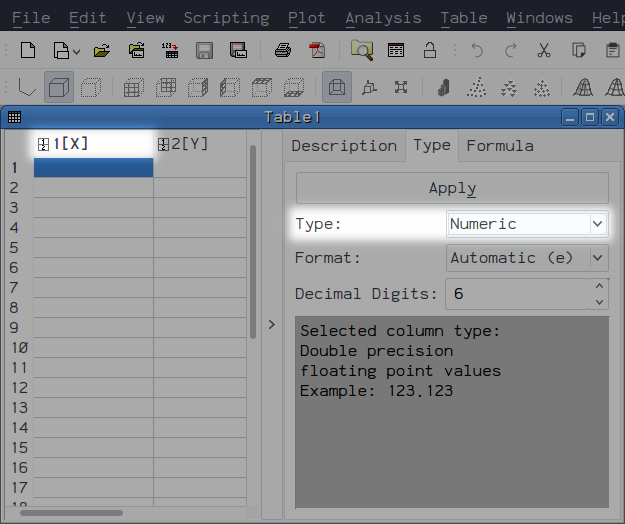
\includegraphics[width=\textwidth]{basico/2coltype.png}

            \caption{Tipo dos dados da coluna}
            \label{fig:basico:coltipo}
        \end{subfigure}
        \caption{Configuração da coluna selecionada}
        \label{fig:basico:config}
    \end{figure}

    \begin{lembrete}
        Lembre-se de pressionar o botão \texttt{Apply} sempre que alterar alguma propriedade da coluna, para realizar as alterações.
    \end{lembrete}
